\chapter{Generative models}


\begin{description}
    \item[Generative task] \marginnote{Generative task}
        Given the training data $\{ x^{(i)} \}$, learn the distribution of the data so that a model can sample new examples:
        \[ \hat{x}^{(i)} \sim p_\text{gen}(x; \matr{\theta}) \]

        \begin{figure}[H]
            \centering
            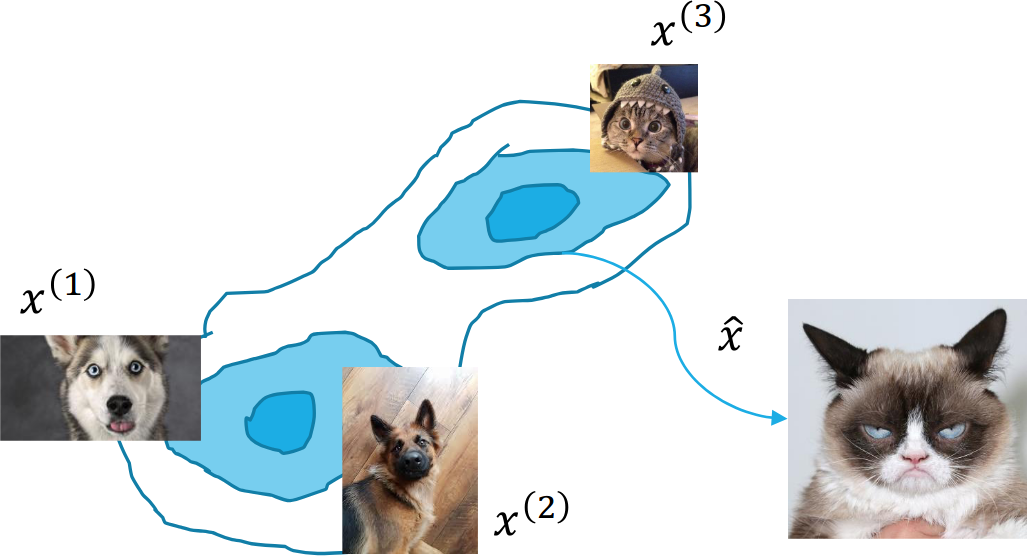
\includegraphics[width=0.4\linewidth]{./img/generative_task.png}
        \end{figure}

        \begin{remark}
            Generative tasks are hard as natural images lay on a low dimensional subspace (i.e., only a tiny subset of all the possible RGB images makes sense).

            \begin{figure}[H]
                \centering
                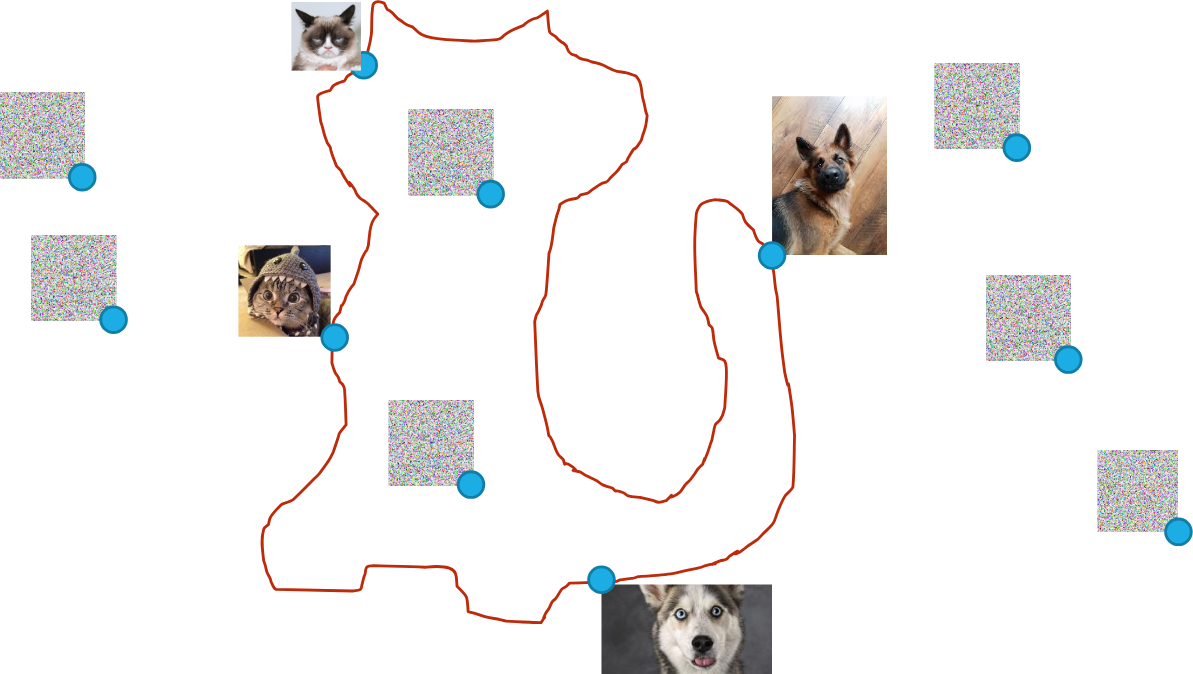
\includegraphics[width=0.6\linewidth]{./img/image_manifold.png}
            \end{figure}
        \end{remark}

    \item[Latent vector] \marginnote{Latent vector}
        Low-dimensional representation to encode an image.

        \begin{example}
            Face expression depends on 42 muscles. A latent representation for different poses of a face can be represented with a 42-dimensional vector.
        \end{example}

        It is assumed that the factors of a latent vector are independent or mildly correlated, and can be sampled from a known distribution.

    \item[Generative model] \marginnote{Generative model}
        Model that takes as input a latent representation and maps it into an output image.
        \begin{figure}[H]
            \centering
            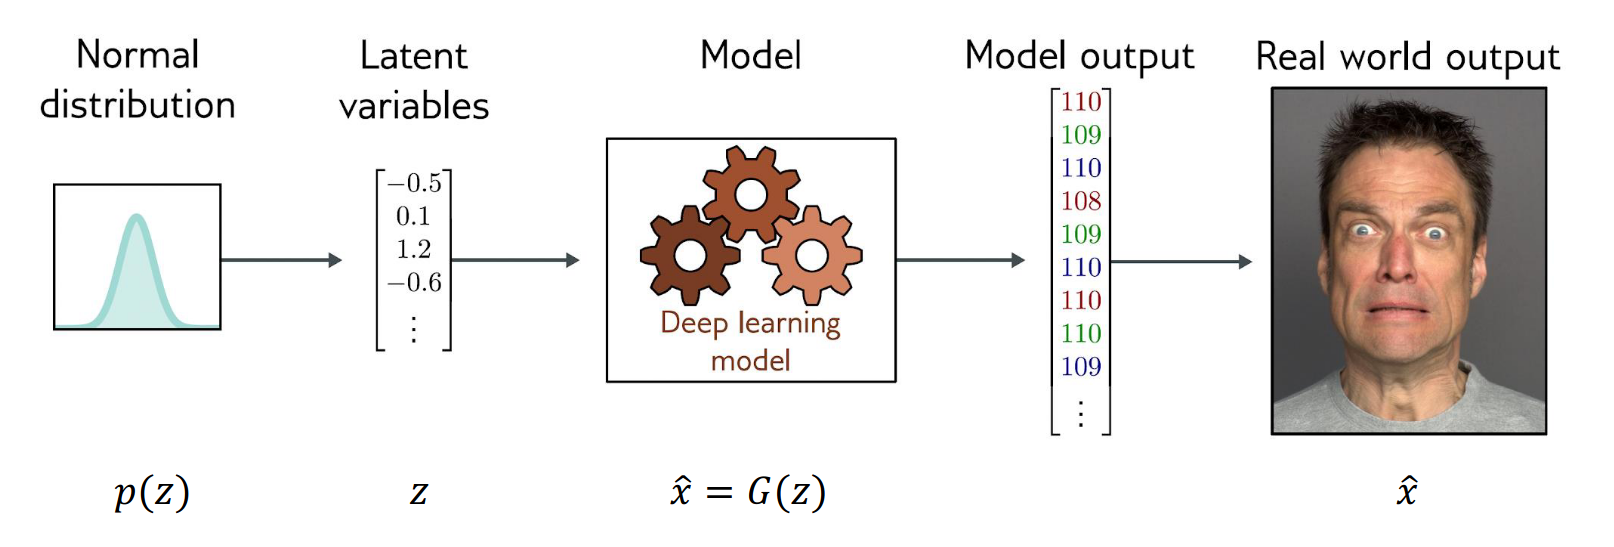
\includegraphics[width=0.7\linewidth]{./img/latent_for_generation.png}
        \end{figure}

        \begin{remark}
            An ideal generative model should have the following properties:
            \begin{itemize}
                \item Be computationally efficient when sampling.
                \item Produce high-quality samples.
                \item Represent the entire training distribution.
                \item Produce a plausible output from any latent input. Smooth changes to the input should be reflected on the output.
                \item Have a disentangled latent space (i.e., changing a dimension of the latent space corresponds to interpretable changes in the output image).
                \item Have the possibility to calculate the probability of the produced images (when the model is probabilistic). 
            \end{itemize}
        \end{remark}
\end{description}



\section{Metrics}

\begin{description}
    \item[Expectation/Expected value] \marginnote{Expectation/Expected value}
        Informally, it is the generalization of the weighted average:
        \[ 
            \mathbb{E}_{x \sim p}[ f(\cdot) ] = \sum_{x \in \mathbb{X}} \prob{x} f(x) 
            \qquad
            \mathbb{E}_{x \sim p}[ f(\cdot) ] = \int_{x \in \mathbb{X}} \prob{x} f(x) \,dx
        \]

        \begin{description}
            \item[Monte Carlo approximation] \marginnote{Monte Carlo approximation}
                Approximation for expectation using $N$ i.i.d. samples drawn from $p(x)$:
                \[ \mathbb{E}_{x \sim p}[f(\cdot)] \approx \frac{1}{N} \sum_{x_i \sim p(x)} f(x_i) \]
        \end{description}

    \item[Self-information] \marginnote{Self-information}
        Given a probability mass function of an event, the self-information of an event $x$ is defined as:
        \[ I(x) = -\log_b(\prob{x}) = \log_b\left( \frac{1}{\prob{x}} \right) \]
        Intuitively, it can be seen as a measure of surprise.

        \begin{example}
            Consider the toss of a fair coin. The self-information for the outcomes are:
            \[ I(\texttt{heads}) = I(\texttt{tails}) = \log_2\left( \frac{1}{0.5} \right) = 1 \]
            If the coin is loaded toward tails with probability:
            \[ 
                \prob{\texttt{heads}} = 0.05 
                \qquad 
                \prob{\texttt{heads}} = 0.95 
            \]
            The self-information is:
            \[ 
                I(\texttt{heads}) = \log_2\left( \frac{1}{0.05} \right) = 4.31
                \qquad
                I(\texttt{tails}) = \log_2\left( \frac{1}{0.95} \right) = 0.07
            \]
        \end{example}
\end{description}